\documentclass{article}
\usepackage[utf8]{inputenc}
\usepackage[serbian]{babel}
\usepackage{hyperref}
\usepackage{placeins}

\title{Klasifikacija podataka prikupljenih u okviru eksperimenta o kratkim sastancima na slepo}
\author{Darinka Zobenica}
\date{}

\usepackage{natbib}
\usepackage{graphicx}

\begin{document}

\maketitle

\section*{Sažetak}
U ovom radu prikazana je klasifikacija podataka prikupljenim u okviru eksperimenta vršenog u Kolumbiji u svrhu naučnog rada o razlikama između polova prilikom biranja partnera.\cite{genderdatingpreferences} Ipak, eksperiment je prikupio mnogo drugih zanimljivih podataka o ispitanicima, te će u ovom radu biti predstavljeni rezultati dobijeni klasifikacijom o uticaju etničke pripadnosti, novčanih prihoda, zajedničkih interesovanja, i razlike u godinama, na izbor partnera.\par
Treba uzeti u obzir da su ispitanici iz SAD i da ne mora da znači da su rezultati relevantni na globalnom nivou, iako se daljim ispitivanjem može utvrditi da jesu.

\tableofcontents
\newpage
\section{Priprema podataka}
Kako korišćeni skup podataka sadrži 190 kolona i 8378 podataka, prvo sam izbacila kolone koje neće biti korišćene. Sačuvane relevantne kolone su:

\begin{itemize}
    \item wave - Pošto je eksperiment ponavljan sa različitim ispitanicima tokom tri nedelje, u koloni wave nalaze se podaci o tome kada se određeni susret desio. Ova kolona ima celobrojne vrednosti od 1 do 21.
    \item age, age\_o - Podaci o uzrastu ispitanika i njihovog partnera za dati sastanak, iskazani kao ceo broj (godina).
    \item race, race\_o - Podaci o izraženoj etničkoj pripadnosti ispitanika i njihovog partnera za dati sastanak, gde brojevi sa sledećeg spiska odgovaraju brojevima u podacima:
    \begin{enumerate}
        \item Negroidna rasa
        \item Evropeidna rasa
        \item Hispano i Latinoamerikanci
        \item Mongoloidna rasa
        \item Američki starosedeoci
        \item Ostali
    \end{enumerate}
    \item samerace - Oznaka da li su ispitanik i trenutni partner iste rase ili ne.
    \item imprace - Koliko je ispitanik označio da mu je rasa bitna u izboru partnera.
    \item int\_corr - Korelacija između interesovanja ispitanika i trenutnog partnera, izvedena na osnovu popunjenog upitnika.
\end{itemize}

Napravila sam dve nove kolone na osnovu već postojećih:

\begin{itemize}
    \item age\_gap - Brojčani podatak dobijen kao apsolutna razlika kolona age i age\_o, koje se odnose na godine prvog i drugog ispitanika, redom.
    \item income\_num - Brojčani podatak dobijen konverzijom niske iz kolone income u broj.
\end{itemize}

Primetila sam da nekoliko kolona koje sadrže kategoričke podatke nemaju jednaku količinu podataka za svaku od kategorija. Kako balansiranje podataka može dovesti do pristrasnosti modela ukoliko nema dovoljno podataka, odlučila sam da izbalansiram samo rasu. Pre balansiranja modeli su favorizovali belce kao najčešću etničku grupu među ispitanicima, a činjenica da je balansiranje poboljšalo preciznost krajnjeg rezultata govori o tome da u ovom slučaju do pristrasnosti nije došlo. Isti postupak nije primenjen na stavke kao što su starost i primanja, zbog manjka podataka za ekstremne vrednosti, a njihove istovremene relevantnosti za rezultate.\par
Tokom preprocesiranja, izbačeni su podaci za wave=12, jer su uslovi eksperimenta tog dana bili specifični (ispitanici su imali limitiran broj ljudi koje su mogli da odaberu da su im se svideli).\par
Za kraj, izbačeni su svi podaci za koje postoji nedostajuća vrednost u bilo kojoj od ovih kolona. Početni skup podataka je konzistentno sadržao isključivo sistemske nedostajuće vrednosti i dozvoljene vrednosti, tako da ništa drugo nije bilo potrebno uraditi.\par
Na sledećoj slici prikazani su korišćeni čvorovi:\\
\begin{figure}[h!]
\centering
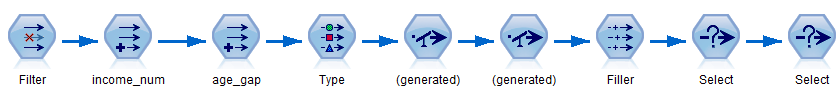
\includegraphics[scale=0.4]{graphics/preprocessing.png}
\caption{Preprocesiranje}
\label{fig:preprocesiranje}
\end{figure}

\section{Klasifikacija}
\subsection{Algoritmi}
\subsubsection{C\&R Tree}
Algoritam C\&R Tree je klasifikacija\cite{ibmcrt} i prediktivna metoda bazirana na strukturi stabla. Slično kao C5.0 algoritam koji će takođe biti korišćen, ova metoda koristi rekurzivno particionisanje da podeli trening podatke u segmente sa sličnim rezultatima. Proces počinje pregledom ulaznih vrednosti u cilju pronalaženja najbolje podele, a kvalitet podele se meri redukcijom mere nečistoće nakon podele. Podela definiše dve podgrupe, od kojih se svaka deli u još dve podgrupe, i tako dalje, dok god se ne ispuni jedan od kriterijuma za zaustavljanje. Sve podele su binarne.\par
Ovaj model je jako dobar za analizu nedostajućih podataka, kao i za korišćenje na velikom broju kolona. Nije potrebno mnogo vremena za trening. Uz to, dobijeni modeli su lakši za razumevanje od nekih dobijenih drugim algoritmima. Za razliku od C5.0, algoritam može da radi sa kontinualnim podacima kao rezultujućim vrednostima, ne samo kategoričkim.
\subsubsection{CHAID}
CHAID algoritam\cite{ibmchaid} je metod izrade stabla odlučivanja koji koristi hi-kvadrat statistiku za određivanje optimalnih podela. CHAID meri koje od ulaznih vrednosti su statistički značajne za određivanje ciljne vrednosti, i bira najznačajniju. Ako ima više od dve kategorije ulaznih vrednosti, one koje su jednako prediktivne se spajaju (inkrementalno redom one koje imaju najmanju razliku). Proces se zaustavlja kada razlika između kategorija dostigne predefinisanu vrednost.\par
CHAID radi za sve tipove ulaznih i izlaznih vrednosti, i pravi proizvoljna stabla (ne isključivo binarna).
\subsubsection{C5.0}
C5.0 algoritam\cite{ibmc50} može da pravi stablo odlučivanja ili pravila pridruživanja. Ovaj model deli uzorak na osnovu atributa koji ima najveću informacionu dobit. Svaki poduzorak definisan prvom podelom se onda ponovo deli i proces se ponavlja dok god poduzorci i dalje mogu da se dele. Na kraju se vrši isecanje tako da se smanji greška zbog preprilagođavanja.\par
Ovaj algoritam radi samo za kategoričke ciljne vrednosti.\par
Prednosti algoritma su iste kao C\&R Tree.
\subsubsection{Neuronska mreža}
Neuronska mreža\cite{ibmnn} je pojednostavljen model načina na koji ljudski mozak procesira informacije. Radi tako što simulira veliki broj povezanih "neurona", podeljenih u ulazni, izlazni, i skriveni sloj. Mreža dodeljuje nasumične težine vezama između neurona, i onda ih optimizuje na osnovu podataka. Optimizacija radi tako što mreža generiše predikciju na osnovu podataka, a onda u zavisnosti od toga da li je predikcija tačna ili ne popravlja odgovarajuće težine grana grafa. Algoritam se zaustavlja kad se ispuni neki od kriterijuma za zaustavljanje.\par
\subsection{Rezultati}
Od svih ispitanika, 83.53\% se nisu svideli međusobno, dok preostalih 16.47\% jesu. Ovo znači da bi naši modeli imali visoku preciznost kad bi uvek pogađali da se par neće svideti jedan drugom, ali nama je cilj da upravo što češće pogodi te slučajeve, čak i po cenu nekog nivoa greške kod onih koji se ne svide jedni drugima.\par
Na sledećoj slici prikazan je deo toka podataka u kome se vrši klasifikacija:
\begin{figure}[h!]
\centering
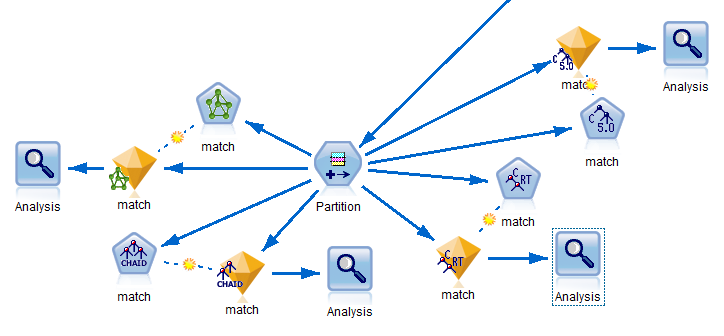
\includegraphics[scale=0.36]{graphics/classification.png}
\caption{Klasifikacija SPSS}
\label{fig:classification}
\end{figure}
\FloatBarrier
\subsubsection{C\&R Tree}
C\&R Tree je procenio da etnička pripadnost i razlike u godinama imaju najveći uticaj na to da li će se dvoje svideti jedno drugom na kratkom sastanku, dok su interesovanja i novčana primanja manje bitni. \par
Najbolje rezultate dobila sam korišćenjem Twoing algoritma. \par
\begin{figure}[h!]
\centering
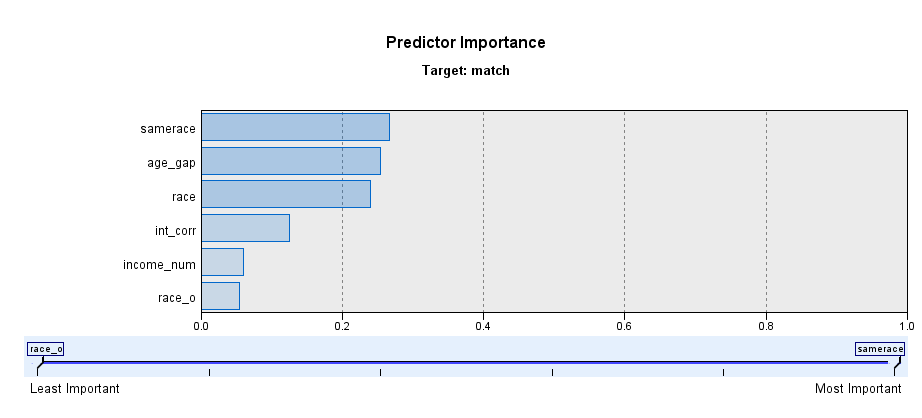
\includegraphics[scale=0.36]{graphics/impcrt.png}
\caption{Uticaj atributa C\&R Tree}
\label{fig:impcrt}
\end{figure}
\FloatBarrier
Klasifikacija je izvršena sa preciznošću od 81.6\% na test skupu, a samo u 33.78\% slučajeva pogađa kada će se dvoje svideti jedno drugom. Zaključujemo da je klasifikacija loše izvršena.
\begin{figure}[h!]
\centering
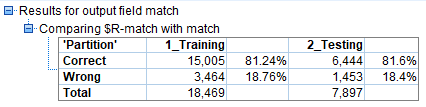
\includegraphics[scale=0.6]{graphics/analcrt.png}
\caption{Analiza modela C\&R Tree}
\label{fig:analcrt}
\end{figure}
twoig
\FloatBarrier
\subsubsection{CHAID}
CHAID algoritam je procenio da su svi atributi jednako važni za predikciju. Model na test podacima ima preciznost od 82.72\%, i pritom u samo 41\% slučajeva pogađa kada će se dvoje svideti jedno drugom. Algoritam je procenio sve atribute kao skoro jednako bitne.
\begin{figure}[h!]
\centering
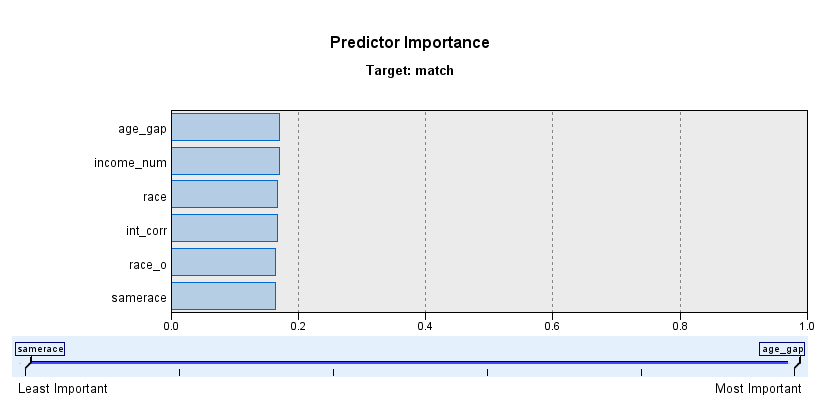
\includegraphics[scale=0.4]{graphics/impchaid.png}
\caption{Uticaj atributa CHAID}
\label{fig:impchaid}
\end{figure}
\begin{figure}[h!]
\centering
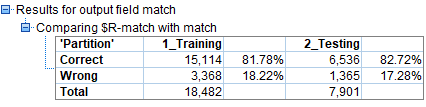
\includegraphics[scale=0.6]{graphics/analchaid.png}
\caption{Analiza modela CHAID}
\label{fig:analchaid}
\end{figure}
\FloatBarrier
\subsubsection{C5.0}
\begin{figure}[h!]
\centering
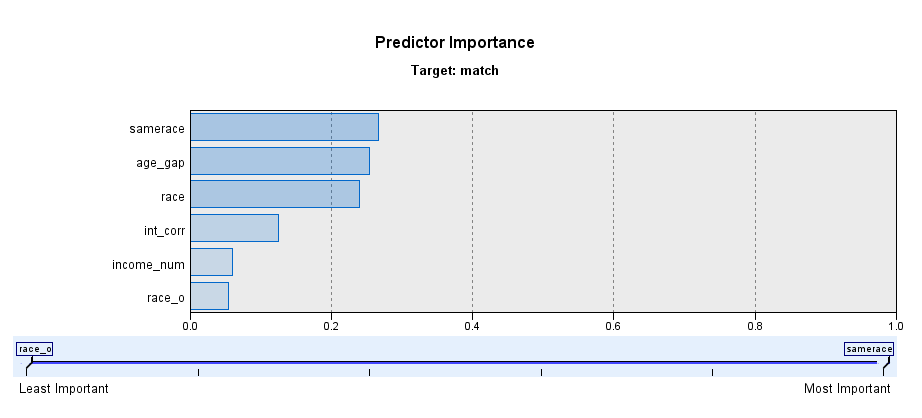
\includegraphics[scale=0.4]{graphics/impc50.png}
\caption{Uticaj atributa C5.0}
\label{fig:impc50}
\end{figure}
\FloatBarrier
Algoritam je procenio da su rasa i razlika u godinama gotovo jednako bitni za izbor partnera, pri čemu je da li su partneri iste rase malo bitniji faktor. Iz dobijenog stabla odlučivanja se može videti da se partneri iste rase češće biraju međusobno, posebno u određenim demografijama. U poređenju s tim, novčana primanja i interesovanja se nisu pokazala kao toliko bitan faktor.\par
\begin{figure}[h!]
\centering
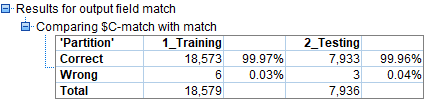
\includegraphics[scale=0.6]{graphics/analc50.png}
\caption{Analiza modela C5.0}
\label{fig:analc50}
\end{figure}
Algoritam C5.0 pokazao je najbolje rezultate, sa čak 99.96\% pogođenih test slučajeva. Prilikom testiranja algoritam je pogrešio samo u 5 primera, od kojih je samo jedan u slučaju kada su se partneri jedan drugom svideli. Ovakve rezultate postigla sam korišćenjem optimizacija boosting i global pruning.
\FloatBarrier
\subsubsection{Neuronska mreža}
Nakon C5.0, neuronska mreža je imala najbolje rezultate, sa 86.83\% pogodaka i čak 57.33\% pogodaka u slučaju kada su se partneri svideli jedno drugom. Kao najbitnije faktore procenila je zajednička interesovanja. Dalji trening nije popravljao dobijene rezultate.
\begin{figure}[h!]
\centering
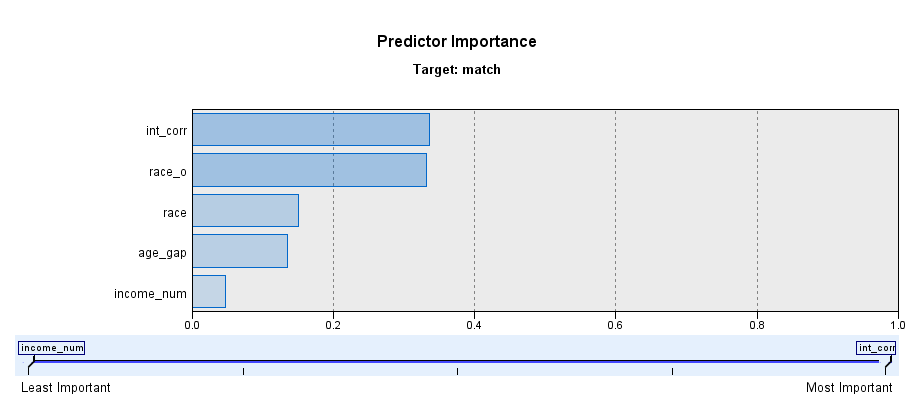
\includegraphics[scale=0.4]{graphics/impnn.png}
\caption{Uticaj atributa Neuronska mreža}
\label{fig:impnn}
\end{figure}
\begin{figure}[h!]
\centering
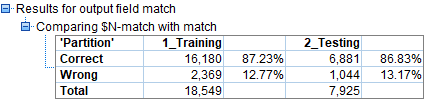
\includegraphics[scale=0.6]{graphics/analnn.png}
\caption{Analiza modela Neuronska mreža}
\label{fig:analnn}
\end{figure}
\FloatBarrier

\section{Zaključak}
Najefikasnijim se pokazao algoritam C5.0 sa čak 99.96\% pogođenih rezultata. Ostali algoritmi su se znatno gore pokazali, pri čemu je C\&R Tree bio najgori.\par
Na osnovu rezultata C5.0 algoritma možemo zaključiti da su za ispitanike u Kolumbiji od testiranih faktora najbitniji godine i etnička pripadnost, dok su zarada i zajednička interesovanja manje bitni.\par


\bibliographystyle{plain}
\bibliography{references}
\end{document}
